\chapter{Results}

In this chapter ve evaluate the simulator the NextGen SPICE library's performance based on the used precision type. We will also compare the our simulator with the ngspice  and SpiceSharp simulator. We will test the performance on the following circuits:

\begin{itemize}
	 \item \texttt{adder} -- a four-bit adder circuit.
	 \item \texttt{astable} -- a simple stable multivibrator.
	 \item \texttt{backtoback} -- the back-to-back diode circuit from the Mike Robbins' paper about using double-double in circuit simulation \cite{circuitlab_dd}.
	 \item \texttt{cfflop} -- a saturating complementary flip flop.
	 \item \texttt{choke} -- circuit containing two diodes used to choke the voltage source.
	 \item \texttt{diffpair} -- simple differential pair.
	 \item \texttt{ecl} -- emmiter coupled logic inverter.
	 \item \texttt{rca3040} -- circuit simulating a RCA3040 wideband amplifier
	 \item \texttt{rtlinv} -- cascade RTL inverters.
	 \item \texttt{sbdgate} -- Shottky-barrier TTL inverter.
	 \item \texttt{ua709} -- circuit simulating the UA 709 opamp.
\end{itemize}

The \texttt{backtoback} circuit is the circuit with two back-to-back diodes and a $1 \mu\Omega$ resistor which was shown back in the introduction chapter in section \ref{chap:intro:dd}. The \texttt{adder} circuit was taken from Andrei Vladimirescu's The SPICE Book \cite{spice_book}, p. 199. Detailed description of the other circuits, including their schematics, can be found in appendix I of the Nagel's Ph.D. thesis \cite{Nagel:M520}. For convenience, we included a copy of his thesis in the attached CD at \texttt{/references/ERL-520.pdf}.

The circuits taken from the Nagel's Ph.D. thesis needed to be slightly modified, because they were intended for SPICE2, which uses different names for some model parameters than SPICE3 (e.g. SPICE2 uses \texttt{CCS} for collector-substrate junction capacitance, SPICE3 and NextGen SPICE library uses \texttt{CJS}). Moreover, the \texttt{.OPTION} statements had to be removed because they are not implemented in our parser. However, no other modifications to the netlists were needed in order to parse them in our library. The actual versions of the netlist files which were used for benchmarks can be found on the attached CD in the \texttt{/examples} folder. 

\section{Comparison of Precision Type Performance}
\label{chap:results-precision}
We have run a transient analysis on these circuits using the double, double-double and quad-double precision types with native implementation Gaussian elimination algorithm. We used the BenchmarkDotNet library to obtain the results shown in the following table. The simulations are grouped by the simulated circuits, also, relevant information about each circuit is included. Times in the table do not include the time spent parsing the circuit, rows with \texttt{NA} mean that the calculation of some timepoint did not converge after 10000 iterations.\footnote{The simulations mentioned in this chapter were run on system with i5-6300HQ 2.30 GHz CPU using .NET Core 2.0.6 (CoreCLR 4.6.26212.01, CoreFX 4.6.26212.01), 64bit RyuJIT, Release mode.}

\begin{center}
	\begin{longtable}{|l|r|r|r|r|}
		\hline
Method &          Mean &         Error &        StdDev & Scaled   \\ \hline \hline
\multicolumn{5}{|l|}{\texttt{adder}: 451 variables, 446 devices (180 BJT transistors), 50 timepoints}  \\ \hline
double  &       NA &       NA &       NA &      ?   \\
double-double  &  9.147 s & 0.2595 s & 0.1716 s &      ?   \\
quad-double  & 86.230 s & 1.3810 s & 0.9134 s &      ?   \\
\hline \hline
\multicolumn{5}{|l|}{\texttt{astable}: 17 variables, 10 devices, 100 timepoints}  \\ \hline
double  &    14.78 ms &  0.1047 ms &  0.0979 ms &   1.00   \\
double-double  &   178.91 ms &  0.6506 ms &  0.5768 ms &  12.11   \\
quad-double  & 1,404.55 ms & 17.1084 ms & 14.2863 ms &  95.04   \\
\hline \hline
\multicolumn{5}{|l|}{\texttt{backtoback}: 7 variables, 4 devices, 1000 timepoints}   \\ \hline
double  &   2.640 ms & 0.0758 ms & 0.0843 ms &    1.00   \\
double-double  &   6.696 ms & 0.0684 ms & 0.0640 ms &   2.54   \\
quad-double  &  46.549 ms & 0.3565 ms & 0.3335 ms &  17.65   \\
\hline \hline
\multicolumn{5}{|l|}{\texttt{cfflop}: 18 variables, 19 devices, 1000 timepoints}  \\ \hline
double  &  16.493 ms & 0.3227 ms & 0.6061 ms &   1.00   \\
double-double  &  57.694 ms & 0.5024 ms & 0.4699 ms &   3.50   \\
quad-double  & 460.006 ms & 7.4204 ms & 6.9410 ms &  27.93   \\
\hline \hline
\multicolumn{5}{|l|}{\texttt{choke}: 11 variables, 8 devices, 100 timepoints}  \\ \hline
double  &    752.0 $\mu{}$s &  14.774 $\mu{}$s &  13.820 $\mu{}$s &   1.00   \\
double-double  &  2,223.9 $\mu{}$s &  44.123 $\mu{}$s &  45.311 $\mu{}$s &   2.96   \\
quad-double  & 17,512.9 $\mu{}$s & 248.354 $\mu{}$s & 220.159 $\mu{}$s &  23.30   \\
\hline \hline
\multicolumn{5}{|l|}{\texttt{diffpair}: 21 variables, 12 devices, 100 timepoints}  \\ \hline
double  &        NA &        NA &        NA  &      ?   \\
double-double  &  8.487 ms & 0.0807 ms & 0.0630 ms &      ?   \\
quad-double  & 65.206 ms & 0.1859 ms & 0.1553 ms &      ?   \\
\hline \hline
\multicolumn{5}{|l|}{\texttt{ecl}: 25 variables, 12 devices, 50 timepoints}  \\ \hline
double  &        NA &        NA &        NA  &      ?   \\
double-double  &  2.282 ms & 0.0191 ms & 0.0179 ms  &      ?   \\
quad-double  & 18.135 ms & 0.4415 ms & 0.7254 ms &      ?   \\
\hline \hline
\multicolumn{5}{|l|}{\texttt{rca3040}: 44 variables, 26 devices, 400 timepoints}  \\ \hline
double  &         NA &       NA &       NA &      ?   \\
double-double  &   150.7 ms & 20.12 ms & 13.31 ms &      ?   \\
quad-double  & 1,286.7 ms & 29.24 ms & 19.34 ms &      ?   \\
\hline \hline
\multicolumn{5}{|l|}{\texttt{rtlinv}: 15 variables, 8 devices, 100 timepoints}  \\ \hline
double  &    549.5 $\mu{}$s &   5.197 $\mu{}$s &   4.607 $\mu{}$s &   1.00   \\
double-double  &  1,632.0 $\mu{}$s &  31.832 $\mu{}$s &  44.625 $\mu{}$s &   2.97   \\
quad-double  & 11,414.4 $\mu{}$s & 152.975 $\mu{}$s & 135.608 $\mu{}$s &  20.77   \\
\hline \pagebreak
\hline
\multicolumn{5}{|l|}{\texttt{sbdgate}: 65 variables, 35 devices, 200 timepoints}  \\ \hline
double  &         NA &       NA &       NA &      ?   \\
double-double  &   130.3 ms & 25.47 ms & 16.85 ms &      ?   \\
quad-double  & 1,273.4 ms & 27.82 ms & 18.40 ms &      ?   \\
\hline \hline
\multicolumn{5}{|l|}{\texttt{ua709}: 61 variables, 39 devices, 125 timepoints } \\ \hline
double  &         NA &       NA &       NA &      ?   \\
double-double  &   123.5 ms & 20.96 ms & 13.86 ms &      ?   \\
quad-double  & 1,244.7 ms & 27.23 ms & 18.01 ms &      ?   \\
\hline	
	\end{longtable}
\end{center}

%fix vspace

\vspace{-1cm}

As seen from the table, using the built-in double type leads to the fastest simulation. However, the simulation of \texttt{adder}, \texttt{diffpair}, \texttt{ecl}, \texttt{rca3040}, \texttt{sbdgate} and \texttt{ua709} did not converge. Because the same circuits converge when enhanced precision types are used, the nonconvergence is probably due to truncation errors during the equation solution, which lead to oscillation around the correct solution, but outside the simulator tolerances. We also ran all these simulations in ngspice simulator successfully without any nonconvergence issues, even though the ngspice uses only standard double precision. We attribute this to the fact that ngspice has been in development for many years and contains many tweaks to ensure convergence.

In terms of simulator output, the output values differ mostly in the 10th significant digit or lower and the data plots for each precision type are visually indistinguishable from each other. The sole exception is the \texttt{backtoback} circuit. In the version where only double precision was used, the truncation errors lead to numerical noise discussed in section \ref{chap:intro:dd} of the introduction chapter. Figure \ref{fig:results:noise} shows the plots for the double and double-double precision type.

\begin{figure}[h]
	\centering
%	\begin{subfigure}
		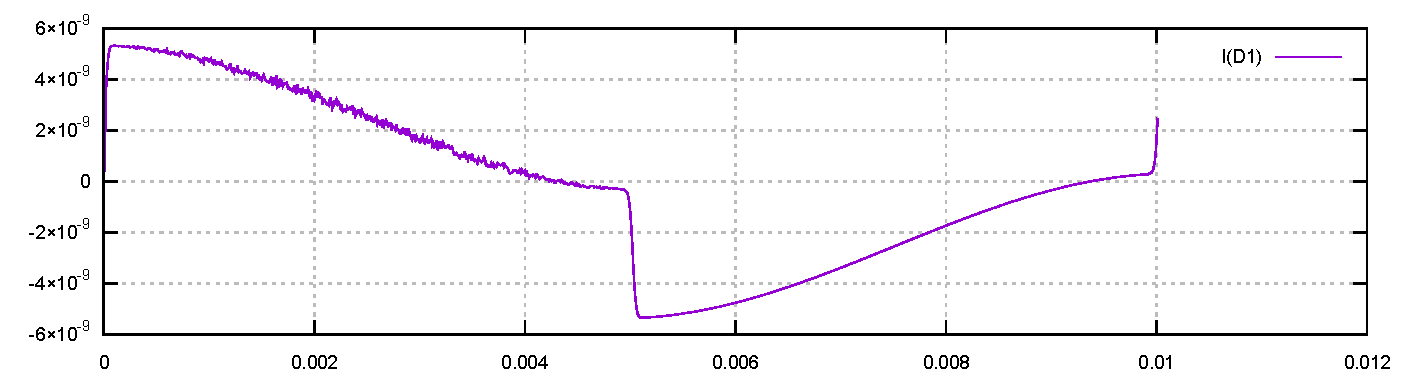
\includegraphics[width=0.9\linewidth]{backtoback-d}
		\caption*{double}
%	\end{subfigure}
%	\begin{subfigure}
		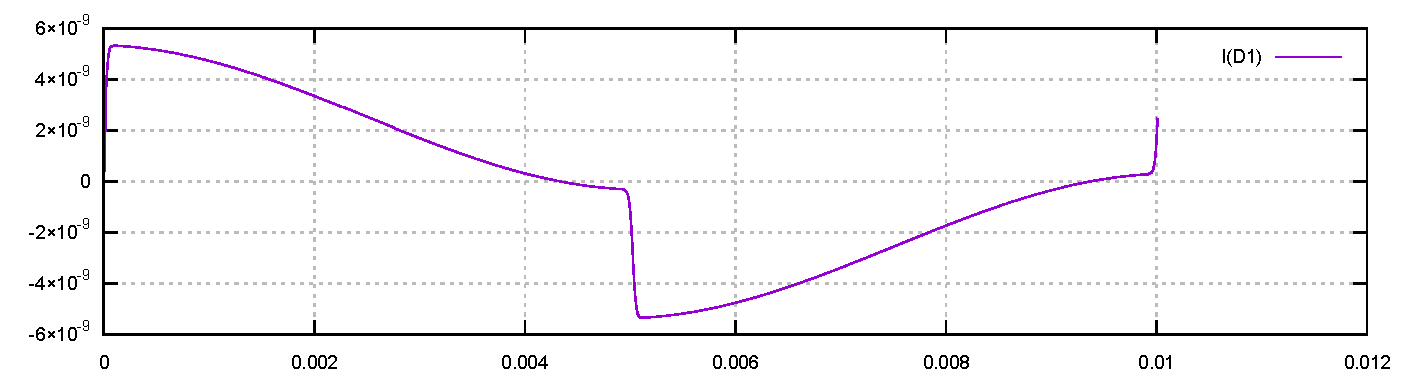
\includegraphics[width=0.9\linewidth]{backtoback-dd}
		\caption*{double-double}
%	\end{subfigure}
	\caption{Comparison of the simulation results for \texttt{backtoback} circuit for double and double-double precision type}
	\label{fig:results:noise}
\end{figure}

Nevertheless, the noise seems to be much smaller than the one produced when simulating the circuit with LTspice (see figure \ref{fig:back-to-back-circuit} back in the introduction chapter).

Using double-double precision over standard double precision helped solve convergence issues in many circuits and helped eliminate noise at the cost of slower simulation speed. From our observations, using quad-double over double-double does not bring any additional benefits (number of iterations needed to simulate the circuit stays the same, double-double already eliminates possible noise from truncation errors in the \texttt{backtoback} circuit) and only slows down the simulation by an order of magnitude. Therefore, we do not recommend using the quad-double type when using the NextGen SPICE library. Instead, we recommend using the double-double precision even though the simulation may be slower than when using only double precision.

In the future versions of the library, we would certainly like to add more convergence aids to ensure convergence even with double precision type. Then the choice of precision type would be based on whether the circuit is expected to be ill-conditioned or not.

\section{Comparison with Ngspice Simulator} 

Following table compares the simulation times of our library with the ngspice simulator. The times listed in the table were obtained using the \texttt{rusage trantime} command in ngspice interactive mode, which lists the time the simulator spent on the transient analysis in seconds with three decimal places. Because of the low resolution of the \texttt{trantime} information, we compared the runs only on the simulations which take several milliseconds. The ngspice simulator was run 5 times and the run times were averaged. The \texttt{adder} circuit was simulated for both 50 timesteps (as in previous section) and 6400 timesteps.

\begin{center}
	\begin{tabular}{|r|r|r|}
		\hline
		Circuit & ngspice & NextGen SPICE (double-double) \\ \hline \hline
		\texttt{cfflop} & 11 ms & 57 ms \\
		\texttt{rca3040} & 8 ms & 150 ms \\
		\texttt{sbdgate} & 6 ms & 130 ms \\
		\texttt{ua709} & 5 ms & 124 ms \\
		\texttt{adder} (50 ns) & 67 ms & 9,147 ms  \\
		\texttt{adder} (6400 ns) & 8.3 s & 898.1 s \\
		\hline
	\end{tabular}
\end{center}

The ngspice simulator is noticeably faster. The ratio of the runtimes of ngspice and that of our library seem roughly proportional to the number of variables in the equation system, in case of the \texttt{adder} circuit with 451 variables, the ngspice simulator was more than 100 times faster. We used the performance profiler integrated in Visual Studio 2017 to find out which parts of our simulator are the slowest. It turns out that the simulator spends more than 95\% of the time solving the equation system. The equation systems for the larger circuits are very sparse, in case of \texttt{adder} circuit, only around 1\% of the matrix entries are nonzero. Because our simulator uses full matrix representation, it spends too much time on multiplying and adding the zero entries. On the other hand, ngspice uses sparse matrix representation which performs only the necessary arithmetical operations.

Therefore, in the next versions of the library, we should implement the sparse matrix representation, and perhaps also consider using different method for solving the equation system to speed up the simulation. Possible choice would be using LU factorization which is also used by ngspice, or even iterative methods like Gauss-Seidel.

\section{Comparison with SpiceSharp}

NextGen SPICE is not the only circuit simulator library for .NET in development. There is SpiceSharp \cite{spicesharp}, whose development started shortly after that of our library. The SpiceSharp is made to resemble the original SPICE3F5, with some modifications to make the source code more appropriate for the .NET platform. Several parts of the source code contain comments with references to the original SPICE3's source and explanation how is it modified.

To compare the user interface of SpiceSharp with that of NextGen SPICE library, consider following code fragment for simulating the simple RLC circuit, which we have simulated in the NextGen SPICE tutorials back in section \ref{chap:tutorial-transient}. We omitted the declarations of outer class and namespace usings for brevity.

\begin{csharpcode}
private static void SpiceSharp()
{
	var circuit = new Circuit(
		new VoltageSource("V1", "1", "0",
			new Pulse(0, 5, 5e-3, 0, 0, 25e-3, double.MaxValue)),
		new Resistor("R1", "1", "2", 50),
		new Inductor("I1", "2", "3", 0.125),
		new Capacitor("C1", "3", "0", 1e-6)
	);
	
	Transient tran = new Transient("TRAN", 0.2e-3, 55e-3);
	Console.WriteLine("Time V(1) V(3) I(VC)");
	
	RealPropertyExport i_v1 = new RealPropertyExport(tran, "V1", "i");
	Console.WriteLine("Time V(1) V(3)");
	tran.OnExportSimulationData += (sender, args) =>
	{
		var time = args.Time;
		var v1 = args.GetVoltage("1");
		var v3 = args.GetVoltage("3");
		var i = i_v1.Value;
	
		Console.WriteLine($"{time} {v1} {v3} {i}");
	};
	
	tran.Run(circuit);
}
\end{csharpcode}

The SpiceSharp user interface is very similar to the SPICE netlist syntax. This means that all devices and nodes are identified by a string. In the NextGen SPICE library, the individual devices can be (optionally) tagged by an arbitrary C\# object.

Another difference is how a circuit is constructed, in case of simple devices, the identifiers of connected nodes are passed to the constructor, and the constructed devices can be passed to the \texttt{Circuit} class constructor. However, the connections for transistors can be only set by calling the \texttt{Connect} instance method, which we found counterintuitive. 

The individual simulations are done by calling a \texttt{Run} method on a dedicated simulation object with the simulated circuit as an argument (see lines 11 and 26 of the source above). Getting the simulation data is a bit tricky. The easiest way to get the node voltages in the individual timepoints is registering a handler on the \texttt{OnExportSimulationData} event (lines 14 to 20). To get e.g. current flowing through the voltage source, one has to use a \texttt{RealPropertyExport} class (line 14) and specify the name of the device and a string name of the property to be extracted. The value of this voltage source current can be then accessed via the \texttt{Value} property during the \texttt{OnExportSimulationData} callback (line 21). 

The SpiceSharp's interface makes heavy use of string values, in the example above we show that getting a current though a device requires knowledge of how the appropriate string identifier. What's worse, the strings are also used to set individual parameters for semiconductor devices. following code fragment is taken from the \texttt{SpiceSharpTest/Models/Semiconductors/DIO/DiodeTests.cs} file from the SpiceSharp's Github repository (version from 4th May 2018).

\begin{csharpcode}
     // Build circuit
	Circuit ckt = new Circuit();
	ckt.Objects.Add(
		CreateDiode("D1", "OUT", "0", "1N914", 
			"Is=2.52e-9 Rs=0.568 N=1.752 Cjo=4e-12 M=0.4 tt=20e-9"),
		new VoltageSource("V1", "OUT", "0", 0.0)
	);
\end{csharpcode}

The \texttt{CreateDiode} method is a helper method which parses the parameter string and sets individual parameters by calling \texttt{SetParameter} method on \texttt{Diode\+Model} class, which internally uses reflection to set appropriate property. The downside of this is that the parameter names cannot be hinted by automatic code completion feature of the IDE (like Intellisense in Visual Studio). These actual object on which the parameters are stored can be accessed, but it takes several casts and is by no means intuitive. Because of this, we consider the interface of our NextGen SPICE library superior to that of SpiceSharp.

Although it's interface is user unfriendly, SpiceSharp implements more circuit analyses and more circuit devices. Also, the implemented models for semiconductor devices are more detailed than those implemented in NextGen SPICE library. We would like to address this in the next version of our library and expand the set of implemented devices and add new analysis types.

We tried to compare the performance of SpiceSharp and the NextGen SPICE library. However, we have had difficulties parsing the netlist files containing the benchmark circuits in the SpiceSharp parser. Some netlist needed to be altered (e.g. \texttt{SIN} source changed to \texttt{SINE}, adding an argument with default value which is not strictly needed by SPICE3, or converting parts of the netlist to lowercase). The SpiceSharp simulator then reported a singular matrix when simulating the \texttt{adder} and \texttt{sbdgate} circuit, and in the circuits which were actually simulated, the SpiceSharp simulator used bigger timestep than we specified. This lead to very shorter simulation times and lower-resolution plots. This makes it difficult to compare the simulators performances. Following table lists measured times and number of timesteps computed.

\begin{center}
	\begin{longtable}{|l|r|r|r|r|r|}
		\hline
Method & Timepoints &        Mean &        Error &       StdDev & Scaled \\ \hline \hline
\multicolumn{6}{|l|}{\texttt{backtoback}} \\ \hline
NextGen SPICE &       1000 &    846.4 $\mu{}$s &    10.319 $\mu{}$s &     9.148 $\mu{}$s &   1.00 \\
SpiceSharp &       5550 & 69,987.3 $\mu{}$s &   565.747 $\mu{}$s &   472.424 $\mu{}$s &  82.70 \\ \hline \hline

\multicolumn{6}{|l|}{\texttt{cfflop}} \\ \hline
NextGen SPICE &       1000 & 59,352.3 $\mu{}$s & 1,151.949 $\mu{}$s & 1,232.573 $\mu{}$s &   1.00 \\
SpiceSharp &         81 &  2,051.9 $\mu{}$s &    29.520 $\mu{}$s &    27.613 $\mu{}$s &   0.03 \\ \hline \hline

\multicolumn{6}{|l|}{\texttt{choke}} \\ \hline
NextGen SPICE &        100 &  2,236.1 $\mu{}$s &    42.844 $\mu{}$s &    40.076 $\mu{}$s &   1.00 \\
SpiceSharp &         73 &    557.4 $\mu{}$s &     7.231 $\mu{}$s &     6.764 $\mu{}$s &   0.25 \\ \hline \hline

\multicolumn{6}{|l|}{\texttt{diffpair}} \\ \hline
NextGen SPICE &        100 &  8,576.7 $\mu{}$s &   165.504 $\mu{}$s &   215.202 $\mu{}$s &   1.00 \\
SpiceSharp &         59 &  1,032.8 $\mu{}$s &    10.943 $\mu{}$s &    10.236 $\mu{}$s &   0.12 \\  \hline \hline

\multicolumn{6}{|l|}{\texttt{rtlinv}} \\ \hline
NextGen SPICE &        100 &  1,569.9 $\mu{}$s &    13.843 $\mu{}$s &    12.271 $\mu{}$s &   1.00 \\
SpiceSharp &         80 &    988.7 $\mu{}$s &    10.505 $\mu{}$s &     9.826 $\mu{}$s &   0.63 \\ \hline \hline
	\end{longtable}
\end{center}

When comparing the runtimes per individual timepoint, the NextGen SPICE is around four times slower, which can be explained by the usage of double-double precision in NextGen SPICE and sparse matrix representation in SpiceSharp. However, when simulating te \texttt{backtoback} circuit, the SpiceSharp needed far more timepoint computations. As seen from in figure \ref{fig:backtoback-spicesharp}, the SpiceSharp does not correctly handle circuits with very small resistors.

\begin{figure}[h]
	\centering
	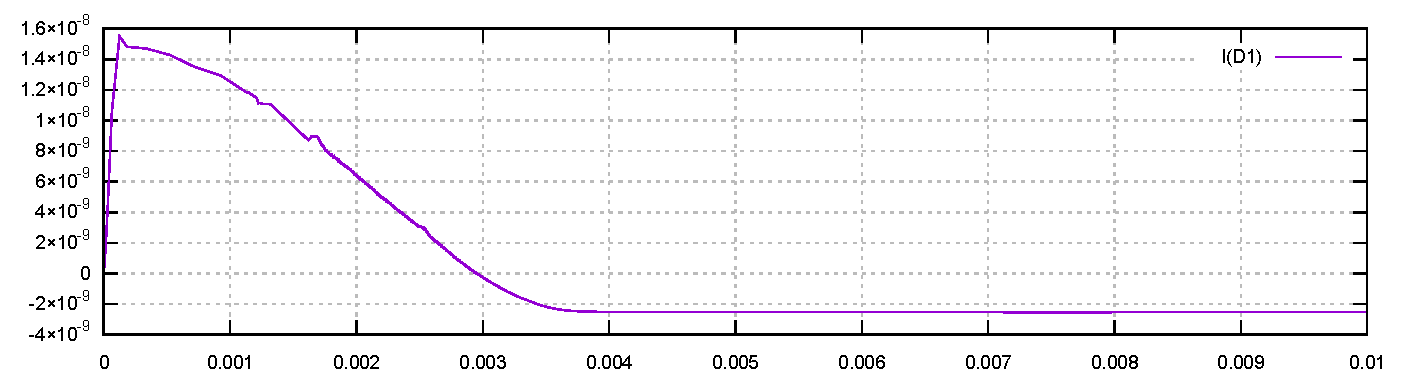
\includegraphics[width=0.9\linewidth]{backtoback-spicesharp.pdf}
	\caption{Plot of the \texttt{backtoback} circuit from SpiceSharp}
	\label{fig:backtoback-spicesharp}
\end{figure}

The plots of other circuits were similar to the ones produced by the NextGen SPICE, although the greater timestep resulted in visible straight regions in the plot. For example, figure \ref{fig:cfflop} shows plot of voltage in \texttt{cfflop} circuit on the \texttt{6} node. At $2\cdot 10^{-7}$ mark, the SpiceSharp output has visible straight edge. Also, the output our NextGen SPICE shows clearly the slight S shape of the slopes when voltage changes. This shape is not clearly visible on the SpiceSharp output.

\begin{figure}[h]
	\centering
	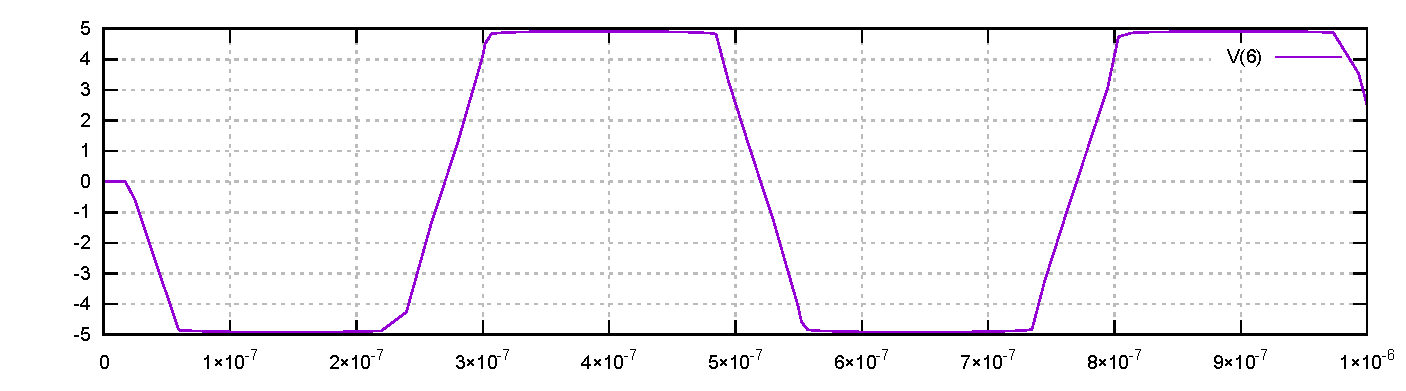
\includegraphics[width=0.9\linewidth]{cfflop-spicesharp}
	\caption*{SpiceSharp}
	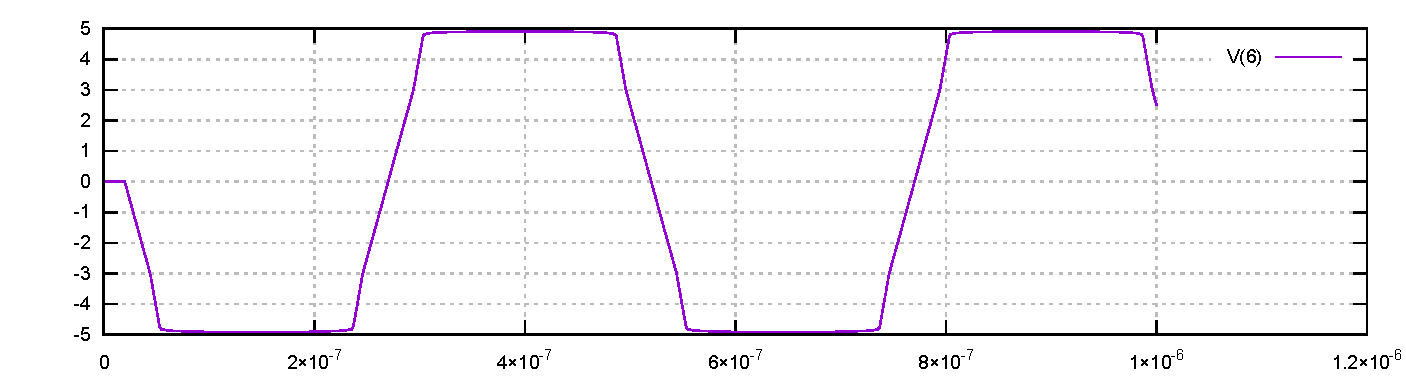
\includegraphics[width=0.9\linewidth]{cfflop}
	\caption*{NextGen SPICE}
	\caption{Comparison of simulation results on the \texttt{cfflop} circuit}
	\label{fig:cfflop}
\end{figure}

\section{Summary}

Considering the measurements listed in this chapter, the representation of equation system and method for solving it is crucial part of the circuit simulator. Our choice of the simplest implementation possible -- full matrix and Gaussian elimination -- caused our simulator to be orders of magnitude slower on large circuits than other circuit simulators. However, thanks to the abstraction we used during the implementation, more appropriate methods can be implemented in future versions of the library. 

In terms of the simulator output, NextGen SPICE produces visually same plots as other circuit simulators, and because of the double-double precision type used, it does not suffer from the noise caused by truncation error during equation system solution.